\documentclass[10pt, journal]{IEEEtran}



%In case you encounter the following error:
%Error 1010 The PDF file may be corrupt (unable to open PDF file) OR
%Error 1000 An error occurred while parsing a contents stream. Unable to analyze the PDF file.
%This is a known problem with pdfLaTeX conversion filter. The file cannot be opened with acrobat reader
%Please use one of the alternatives below to circumvent this error by uncommenting one or the other
%\pdfobjcompresslevel=0
%\pdfminorversion=4

% See the \addtolength command later in the file to balance the column lengths
% on the last page of the document

% numbers option provides compact numerical references in the text.
% \usepackage{natbib}
\usepackage{times}
\usepackage{multicol}
\usepackage[bookmarks=true]{hyperref}
\usepackage{xcolor}
\usepackage{hyperref}
\usepackage{amsmath, amssymb}
\usepackage{amsfonts}
\usepackage{graphicx}
\usepackage{siunitx}
\usepackage{standalone}
\usepackage{booktabs}
\usepackage[ruled,vlined,linesnumbered]{algorithm2e}
\usepackage{mdframed}
\usepackage{fancyvrb}
\usepackage{soul}
\usepackage{dsfont,mathabx}
\usepackage{array, booktabs}
\usepackage{threeparttable}
\usepackage{multirow}

\usepackage{subfigure}
\usepackage{amsthm}
\newtheorem{theorem}{Theorem}
\newtheorem{lemma}[theorem]{Lemma}
\theoremstyle{definition}
\newtheorem{remark}{Remark}
\newtheorem{example}{Example}
\newtheorem{problem}{Problem}
\newtheorem{definition}{Definition}

% GENERAL
\newcommand{\todo}[1]{\textcolor{red}{TODO: #1}}
\newcommand{\improve}[1]{\textcolor{cyan}{IMPROVE: #1}}
\newcommand{\note}[1]{\textcolor{blue}{NOTE: #1}}
\newcommand{\question}[1]{\textcolor{orange}{Q: #1}}
\newcommand{\todoliu}[1]{\textcolor{green}{TODOLIU: #1}}
\newcommand{\noteliu}[1]{\textcolor{green}{NOTELIU: #1}}

%%%%%%%%%%%%%%%%%%%%%%%%%%%%%%%%%%%%%%%%%%%%%%%%%%%%%%%
%%%%


\title{
Supporting materials
} 
\begin{document}

%%========================================
\maketitle
%==============================
%==============================

\section{MILP Formulation}
Give a poset $P=(\Omega,\preceq_{\varphi},\neq_{\varphi})$, where $\Omega$ is a sequence of
subtasks, and~$\preceq_{\varphi}$, $\neq_{\varphi}$ are the partial relations
to describe the relative ordering between the subtasks.
Furthermore, $\omega_1\preceq_{\varphi}\omega_2$ means subtask $\omega_2$ should be
started after $\omega_1$ is started,
and $\omega_1\neq_{\varphi}\omega_2$ means that the execution of $\omega_1,\omega_2$ should not have intersection.
A team of agents is deployed to execute these subtasks under the constraints of
$\preceq_{\varphi},\neq_{\varphi}$ in the given workspace, e.g., as shown in Fig.~\ref{fig:workspace}.
Additionally, the agents are heterogeneous with three different types~$V_f,V_l,V_s$,
e.g., different velocities and functionalities.
For any subtask~$\omega_j\in\Omega$, it needs a particular combination of
different collaborators as specified in Table~\ref{fig:symbols}.
The objective function is to minimize the maximum execution time of
all subtasks in~$\Omega$, i.e., the makespan of the complete plan.
In particular, given the definition of variables in Table~\ref{tab:variables},
the Mixed Integer Linear Program (MILP) for solving this problem is formulated as follows.
Similar formulation can be found in~\cite{luo2021temporal, jones2019scratchs},
but with different objective function and different way of modeling the relative constraints.
The objective function is given by:
\begin{table}[t]
	\centering
	\caption{Description of related regions and agent actions.}
	\label{fig:symbols}
	\begin{tabular}{|c|m{0.5\columnwidth}|c|}\hline
		\textbf{Proposition} & \textbf{Description}\centering & \textbf{Duration} [s]\\ \hline
		$\texttt{p}_1,\cdots,\texttt{p}_{34}$ & $34$ PV panels. & $\backslash$ \\ \hline
		$\texttt{b}$ & Base stations for all agents to park and charge. & $\backslash$ \\ \hline
		$\texttt{t}_1,\cdots,\texttt{t}_7$ & $7$ transformers. & $\backslash$ \\ \hline
		$\texttt{temp}_{\texttt{p}_i,\texttt{t}_i}$ &
		Measure temperature of panel~$\texttt{p}_i$ and transformer $\texttt{t}_i$.
		Requires one~$V_f$. & 10 \\ \hline
		$\texttt{sweep}_{\texttt{p}_i}$& Sweep debris around any panel~$\texttt{p}_i$.
		Requires one $V_s$. & 190\\ \hline
		$\texttt{mow}_{\texttt{p}_i,\texttt{t}_i}$ &
		Mow the grass under panel~$\texttt{p}_i$ or transformer~$\texttt{t}_i$.
		Requires one $V_s$. & 190\\ \hline
		$\texttt{fix}_{\texttt{t}_i}$ &
		Fix malfunctional transformer~$\texttt{t}_i$.
		Requires one $V_l$ and one $V_s$ & 72\\ \hline
		$\texttt{repair}_{\texttt{p}_i}$ &
		Repair broken panel~$\texttt{p}_i$.
		Requires one $V_s$ to repair and two $V_f$ to guide. & 576\\ \hline
		$\texttt{wash}_{\texttt{p}_i}$ &
		Wash the dirt off panel~$\texttt{p}_i$.
		Requires one $V_l$ to wash and one $V_f$ to monitor the progress. & 565\\ \hline
		$\texttt{scan}_{\texttt{p}_i,\texttt{t}_i}$ &
		Build 3D models of panel~$\texttt{p}_i$ or transformer~$\texttt{t}_i$
		for inspection. Requires three $V_f$. & 95\\ \hline
	\end{tabular}
\end{table}
\begin{figure}
	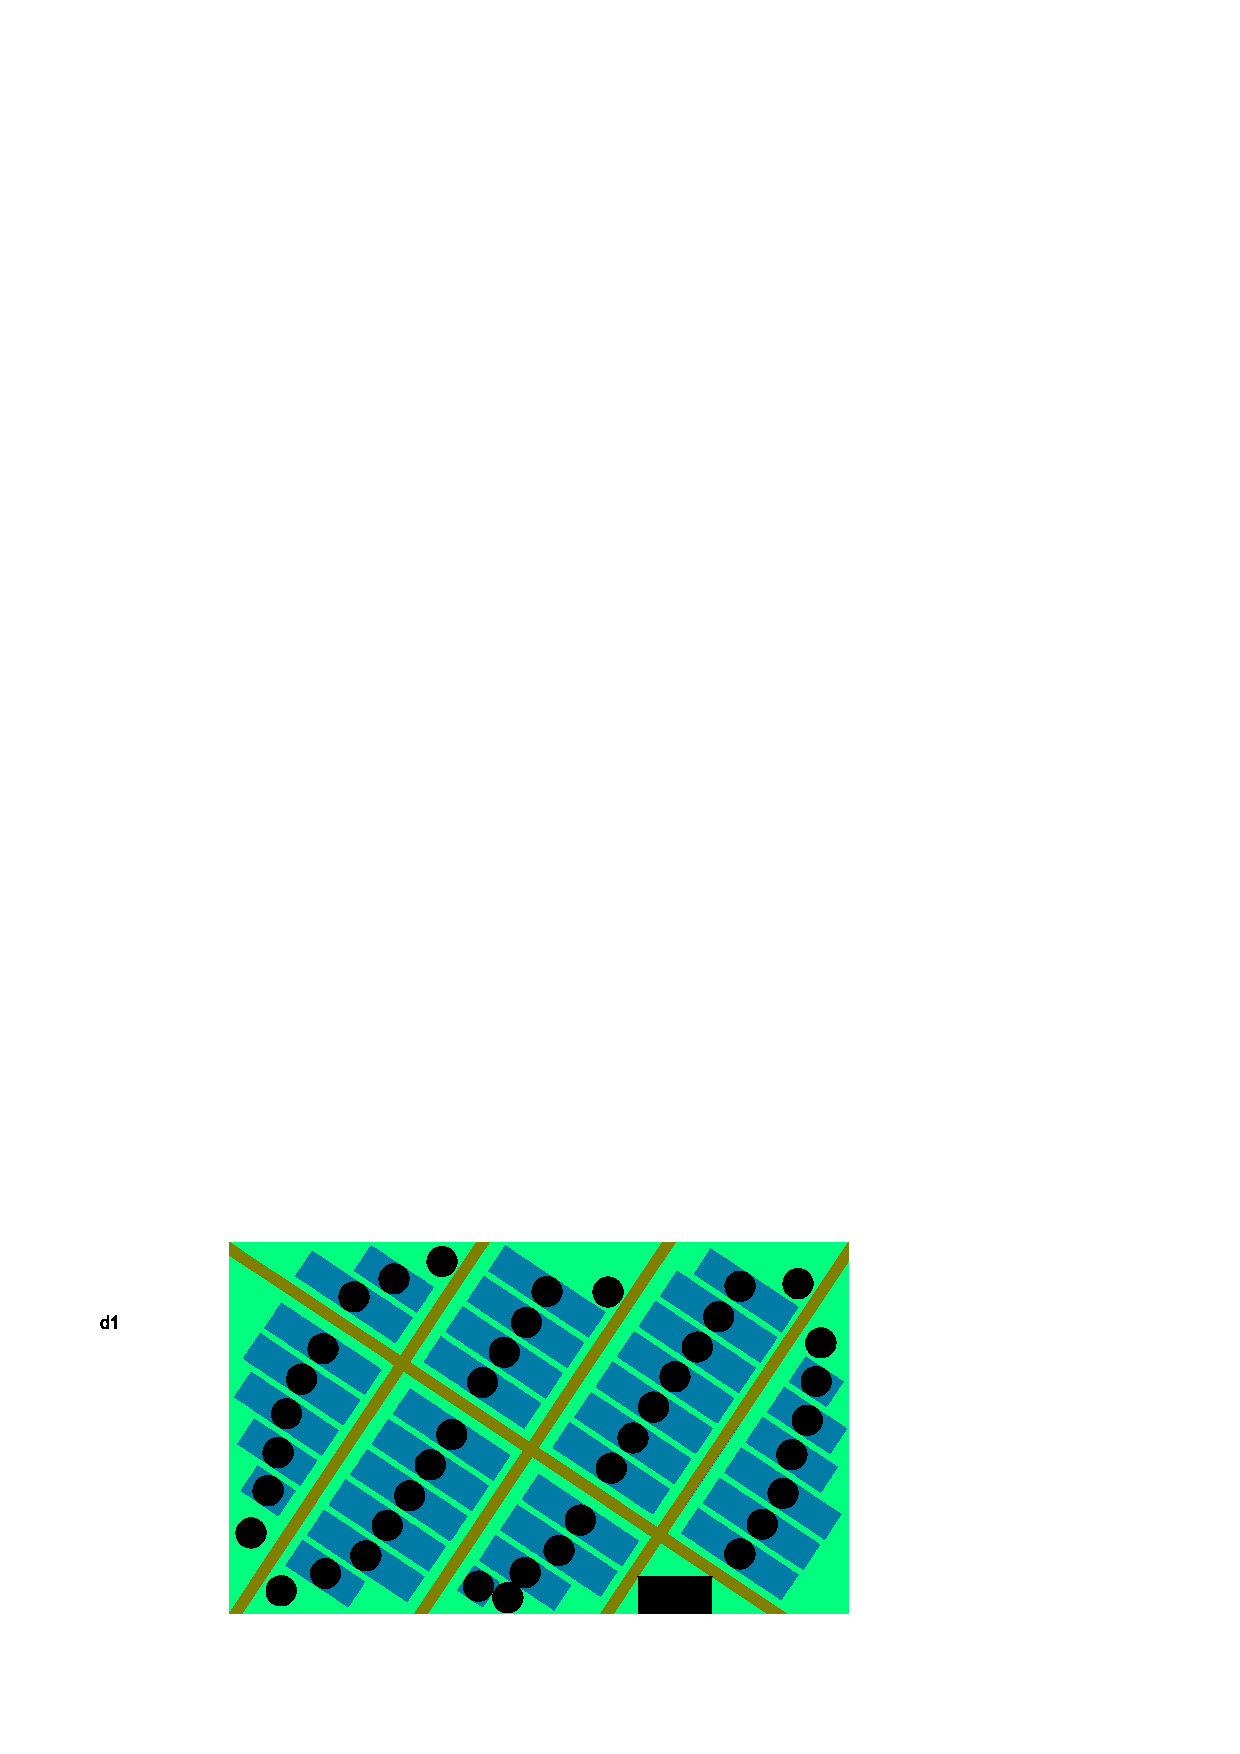
\includegraphics[width=0.36\textheight]{figures/background.pdf}
	\caption{The workspace layout of the simulated PV farm.}
	\label{fig:workspace}
\end{figure}

\begin{table}[t]
	\begin{tabular}{|l|p{0.5\columnwidth}|p{0.2\columnwidth}|}\hline
		Variable &\multicolumn{2}{c|}{ Variable definition }\\\hline
		Name & definition & range \\
		$P$ & partial order set& \\
		$m$  & number of agents & $\mathcal{N}$\\
		$n$ & number of tasks & $\mathcal{N}$ \\
		$i$ & agent $i$ & $i\leq n$\\
		$j$ & task $j$ & $j\leq m$	\\
		$k$ & order of tasks & $j\leq m$\\
		$o$ & number of serves type agent can provide & $ \mathcal{N}$\\
		$l$ & order of tasks & $j\leq o$\\
		$r$ & the ID of tasks set in $\neq$ & $\mathcal{N}$\\
		$\Omega$ & set of subtasks &\\
		$S^r$& a set of tasks belong to $\neq$ &\\
		$q^r_{j_1,j_2}$ &task $j_1$ execute in front of $j_2$ or not& $\{0,1\}$\\
		$T_b$ & a pretty large number as time budget & $T_b>0$ \\
		$r_{i,j,k,l}$ & agent $i$ execute task $j$ providing serve $l$ in the order $k$ & $\{0,1\}$\\
		$t_j$ & begin time of task $j$ & $t_j>0$ \\
		$p_j$ & continue time of task $j$ & $p_j >0$\\
		$a_{j,l}$ & number of servey $l$ task $j$ needed. & $\mathcal{N}$\\
		$b_{i,l}$ & type of servey $l$ that agent $i$ can provide & $\{0,1\}$ \\
		$v_i$ & velocity of agent $i$ &   $v_i>0$\\
		$dis_{j_1,j_2}$ & distance from task $j_1$ to task $j_2$ &  $dis_{j_1,j_2}>0$\\
		$dis_{i,j}$ & distance from initial $i$ to task $j$ & $dis_{i,j}>0$\\\hline
	\end{tabular}
	\centering
	\caption{Definition of variables used in the MILP.}
	\label{tab:variables}
\end{table}
\begin{equation}
\min_{r_{i,j,k,l}, t_j,q_{j_1,j_2}}  \max(t_j+p_j),
\label{0}
\end{equation}
is the objective function.
The following constraints should be satisfied.
Firstly, the $\preceq_{\varphi}$ constraints are enforced by
\begin{equation}
t_{j_1}+p_{j_1}\leq t_{j_2}, \quad  \forall (j_1,j_2)\in \preceq_{\varphi};
\label{1}
\end{equation}
the $\neq_{\varphi}$ constraints are enforced by:
\todoliu{update}
\begin{equation}
 t_{j_1}+p_{j_1}-q^l_{j_1,j_2}T_b\leq t_{j_2}, \forall S^l=\{j_1,j_2,\cdots,j_n\}\subseteq \neq_{\varphi}
 \label{1.5}
\end{equation}

\begin{equation}
\sum_{j_1,j_2\in S^l}q_{j_1,j_2} \leq |S^l|(|S^l|-1)-1, \forall S^l=\{j_1,j_2,\cdots,j_n\}\subseteq \neq_{\varphi}
\label{1.8}
\end{equation}

Furthermore, the required subtasks for each task~$j$ should be satisfied:
\begin{equation}
\sum_{i=1}^{m}\sum_{k=1}^{n}r_{i,j,k,l}b_{i,l}= a_{j,l},   \quad \forall j,l;
\label{2}
\end{equation}
Each agent can only provide the subtasks within its capability:
\begin{equation}
r_{i,j,k,l}\leq b_{i,l},   \quad \forall i,j,k,l;
\label{3}
\end{equation}
Each agent can execute one task no more than once:
\begin{equation}
\sum_{k=1}^{n}\sum_{l=1}^{o}r_{i,j,k,l} \leq 1,\quad   \forall i,j;
\label{4}
\end{equation}
Each agent at any time can execute no more than one task:
\begin{equation}
\sum_{j=1}^{m}\sum_{l=1}^{o}r_{i,j,k,l} \leq 1,\quad    \forall i,k;
\label{5}
\end{equation}
Each agent can execute $k+1$-th task only after it has executed $k$-th task:
\begin{equation}
  \sum_{j=1}^{m}\sum_{l=1}^{o}r_{i,j,k,l} - \sum_{j=1}^{m}\sum_{l=1}^{o}r_{i,j,k+1,l}
  \leq  0,    \quad\forall i,k<m-1;
\label{6}
\end{equation}
Each agent should obey its motion and action model:
\begin{equation}
\begin{aligned}
&t_{i_2}-t_{i_1} -M\sum_{l=1}^o r_{i,j_1,k,l}-M\sum_{l=1}^o r_{i,j_2,k+1,l}  \geq\\
& dis_{j_1,j_2}/v+p_{i_1}-2M, \quad   \forall i,j;
\end{aligned}
\label{7}
\end{equation}
\begin{equation}
t_{i} -M\sum_{l=1}^o r_{i,j,1,l} \geq dis_{i,j}/v-M, \quad  \forall i,j;
\label{8}
\end{equation}
With these constraints mentioned, the associated MILP is completed.
Unfortunately, the required number of bool variables
is $MN^2$, the complexity of solving the underlying MILP
is exploding as~$M$ and $N$ increase.



\section{Alternative Lower Bound}
\label{lower bound method}
In this section,
another method to compute the lower bound is proposed here,
which is more complex than the one proposed in the article.
But it can provide more accurate estimate of the lower bound,
particularly, it performs better when the number of agents and subtasks are small.
Instead of the original conditions in~\eqref{0}~\eqref{8},
a more relaxed version is used here.
More specifically, the distance cost is replaced by the time bound~$t_{low}$
as the minimum time for any agent to reach any goal region.
The lower bound consists of two parts:
the first part is to calculate the exact finishing time of all currently assigned tasks;
the second part is to estimate the makespan based on the current boundary condition.
In particular,
the set of used variables is summarized in Table~\ref{tab:variables2}.
Furthermore, the objective function is given by:
$$ \min_{t_{j_a}} \quad \max(t_{j_a}+p_{j_a}),$$
and the partial ordering constraints are given by:
\begin{equation}
t_{j_{a1}} + p_{j_{a1}}< t_{j_{a2}},   \quad \forall j_{a1}, j_{a2} \in P , j_{a1} \in N_a, j_{a2} \in N_a;
\label{9}
\end{equation}
when task $j$ is the first task of agent $i$, the motion constraint is given by:
\begin{equation}
dis_{i,j_a}/v_i+ p_{j_a}< t_{j_a};
\label{10}
\end{equation}
when task $j_{a2}$ is the subsequent task after task $t_{a1}$ of agent $i$,
the motion constraint is given by:
\begin{equation}
dis_{j_{a1},j_{a2}}/v_i+ p_{j_{a1}}+t_{j_{a1}}- t_{j_{a2}}<0;
\label{11}
\end{equation}
then $t_{i0}$ can be computed as the time each agent finishes
executing all assigned tasks
and starts to execute the remaining unassigned tasks.
$t_{j_a}$ is the time when the execution of task~$j_a$ is finished by agent~$i$.
Denote by~$T_i$ the set of tasks assigned to agent $i$, which yields the
computation of~$t_{i0}$ as follows:
\begin{equation}
t_{i0} = \max{\{t_{j_a}\}},    \quad {j_a}\in T_i;
\label{12}
\end{equation}

\begin{table}[t]
	\begin{tabular}{|l|p{0.5\columnwidth}|p{0.2\columnwidth}|}\hline
		Name & Variable definition & range \\\hline
		$P$ & partial order set& \\
		$M$  & number of agents & $\mathcal{N}$\\
		$\mathcal{M}$  & agent set & \\
		$N_a$ & set of assigned tasks &  \\
		$N_u$ & set of unassigned tasks &  \\
		$T_i$ & assigned tasks for agent $i$ &  \\
		$n_u$ & number of unassigned tasks & $\mathcal{N}$ \\
		$t_{j_a}$ & finished time of assigned tasks & $t_{j_a}>0$\\
		$\Omega$ & anchor function &\\
		$r_{i,j}$ & agent $i$ execute task $j$ & $\{0,1\}$\\
		$t_{i0}$ & begin time of agent $i$ & $t_i>0$ \\
		$t_i$ & end time of agent $i$ & $t_i>0$ \\
		$p_j$ & continue time of task $j$ & $p_j >0$\\
		$p'_j$ & estimate continue time of task $j$ & $p_j >0$\\
		$a_{j}$ & number agent task $j$ needed. & $\mathcal{N}$\\
		$v_i$ & velocity of agent $i$ &   $v_i>0$\\
		$dis_{j_1,j_2}$ & distance from task $j_1$ to task $j_2$ &  $dis_{j_1,j_2}>0$\\
		$dis_{i,j}$ & distance from initial $i$ to task $j$ & $dis_{i,j}>0$\\\hline
	\end{tabular}
	\centering
	\caption{variable definition}
	\label{tab:variables2}
\end{table}
For the remaining tasks, the final lower bound is modified by replacing the
task executing time~$p_j$ with the minimum possible motion cost~$p'_j$:
\begin{equation}
  p'_j = \min{\{\frac{dis_{i,j}}{v_i}, \frac{dis_{j_1,j_2}}{\max_i\, {v_i}}\}}+p_j,
  \quad \forall j\in N_u, \forall i \in \mathcal{M};
\label{13}
\end{equation}
Thus, the objective function and constrains are reformulated as follows:
\begin{equation}
\min_{r_{i,j},t_i} \;\max\, \{t_i\}
\label{14}
\end{equation}
the number of collaborators for each subtask is enforced by:
\begin{equation}
\sum_{i=1}^{m}r_{i,j} = a_{j},\quad  \forall j \in N_u;
\label{15}
\end{equation}
the relaxed constraint on motion and task executing time is given by:
\begin{equation}
\sum_{j=1}^{n}r_{i,j}p'_j +t_i > t_{i0}, \quad \forall i \in \mathcal{M},
\label{16}
\end{equation}
and $r_{i,j}$ is a boolean variable which is $1$ if task $j$ is assigned to agent $i$,
$0$ otherwise:
\begin{equation}
r_{i,j} \in\{0,1\}.
\label{17}
\end{equation}
The complexity of the first part is $O(N_a)$, while the complexity of
the second part is $O(N_u\cdot M)$.
Compared with~\eqref{0}, the ordering relations among subtasks are ignored
thus the poset constraint is neglected. In addition,
for each subtask, the constraints in \eqref{2}-\eqref{4} are removed
and only the constraint in~\eqref{15} is kept.
Also, a collaborative task is not required to be executed by the collaborators
at same time, thus the actual completion time is smaller.

\todoliu{
More specifically, let the current node be~$\nu$,
the set of unfinished subtasks is given by~$\Omega^-_\nu$ in~\eqref{eq:node-tasks}.
The first lower bound~$\underline{T}_{\nu,1}$ on the makespan
to accomplish~$\Omega^-_\nu$ is computed via analyzing the poset
graph~$\mathcal{G}_{P_\varphi}=(\Omega,\, E,\, R)$ in~\eqref{def:poset-graph}.
In particularly, consider the directed
graph~$\mathcal{G}'_{P_\varphi}=(\Omega'_\nu,\, E\cap R )$,
where~$\Omega'_\nu$ is the set of nodes associated with the unfinished subtasks,
and the set of edges contains the edge $(\omega',\,\omega)$ that belongs to
both~$\preceq_{\varphi}$ and~$\neq_{\varphi}$.
Then, starting from the set of root nodes that does not have parent nodes,
a BFS procedure is used to traverse all nodes in the graph~$\mathcal{G}'_{P_\varphi}$.
Denote by~$\Gamma^-_{\nu}=\{\tau_{\omega_f,\omega_g}\}$ the set of paths
from any root node~$\omega_f$ to any other node~$\omega_g$ in the graph.
Then, the first lower bound~$\underline{T}_{\nu,1}$ on the makespan is given by
\begin{equation}\label{eq:lower-bound-1}
\underline{T}_{\nu,1} (\nu,\,P_{\varphi})=\textbf{max}_{\tau\in \Gamma^-_\nu} \, \{T_{\tau}\},
\end{equation}
where~$T_{\tau}$ is the accumulated duration
of path~$\tau=\omega_0\omega_1\cdots \omega_P$, i.e., $T_\tau=\sum_{p=1}^PT_{\omega_p}$.
In other words, the lower bound~$\underline{T}_{\nu,1}$ assumes that
there are as many agents as needed for the sub-tasks, while the partial ordering
constraints for the subtasks are ensured.
Secondly, another lower-bound~$\underline{T}_{\nu,2}$ is estimated by
ignoring the partial ordering constraints:
\begin{equation}\label{eq:lower-bound-2}
\underline{T}_{\nu,2} (\nu,\,P_{\varphi})=\frac{\sum_{\omega\in \Omega^-_{\nu}}
	T_{\omega} N_{\omega}}{N},
\end{equation}
where~$T_{\omega}$ and~$N_{\omega}$ are the duration and number of agents required
for subtask~$\omega\in \Omega^-_\nu$ as defined in~\eqref{eq:node-makespan}.


Consequently, the lower bound on the makespan of all solutions rooted from~$\nu$
is given as the minimum of these two lower bounds above:
\begin{equation}\label{eq:lower-bound}
\underline{T}_\nu = \texttt{lower\_bound}(\nu,\,P_{\varphi})
= \min\,\{\underline{T}_{\nu,1},\, \underline{T}_{\nu,2}\},
\end{equation}
which can be computed efficiently.
It is worth noting that the task assignments associated with~$\underline{T}_\nu$
above is infeasible as it either violates the partial ordering constraints or
the current agent capacities.

}


\section{Details for Numerical Simulation}
\subsection{Planner and Controller}
Each agent is governed by a two-level path planner:
the high-level planner relies on the $A^\star$ method to find the
discrete sequence of waypoints from any initial position to the goal position;
the low-level planner is a simple P-controller with~$RVO$ for collision avoidance.
The agent synthesizes the discrete path first with high level planner,
then uses the lower-level planner to navigate the robot between waypoints.
The transition function between the regions is different among the agents, e.g.,
the UAV can move freely without considering any obstacles,
while the UGVs are restricted from the areas around the PV panels and off-road obstacles.
The collision avoidance mechanism via~$RVO$ is only activated
when the distance between any two agents is smaller than a threshold.

There are three types of agents: $V_f$, $V_s$, $V_l$:
$V_f$ is a quadrotor with model Crazyflie $2.0$,
which has a onboard navigation controller.
All UAVs have the same height and can only move in the $x,y$ plane;
$V_s, V_f$ are both four-wheel-driven car with  MecanNum wheels, with
a simple onboard navigation controller for rotation and translation.


\subsection{Additional Figures}
This section contains the figures illustrating the simulation results
in Section VIII-A,
of the original article, which were omitted for lack of space.

Fig.~\ref{fig:poset_graph1}-\ref{fig:gantt_task1} are the poset graph, the BnB search process,
and the final execution plan for task~$\varphi_1$;
while Fig.~\ref{fig:poset_graph2}-\ref{fig:gantt_task2} are for task~$\varphi_2$.
\begin{figure}[htbp]
		\centering%
		\includegraphics[width =0.18 \textwidth]{figures/simulation/task1/ipe_poset_graph.pdf}
		\caption{Poset graph of task $\varphi_1$. }
                \label{fig:poset_graph1}
\end{figure}

\begin{figure}[htbp]
	\centering
	\includegraphics[width =0.45\textwidth]{figures/simulation/task1/bnb_search1.pdf}
	\caption{ BnB search process of $\varphi_1$.}
        \label{fig:hesse_task1}
\end{figure}

\begin{figure}[htbp]
		\centering
\includegraphics[width =0.43\textwidth]{figures/simulation/task1/gantt_graph.pdf}
\caption{Gantt graph of optimal task assignment in $\varphi_1$.}
\label{fig:gantt_task1}
\end{figure}

%===========================

\begin{figure}[htbp]
		\centering%
\includegraphics[width =0.3\textwidth]{figures/simulation/task2/ipe_poset_graph.pdf}
\caption{Poset graph of task $\varphi_2$.}
\label{fig:poset_graph2}
\end{figure}

\begin{figure}[htbp]
		\centering
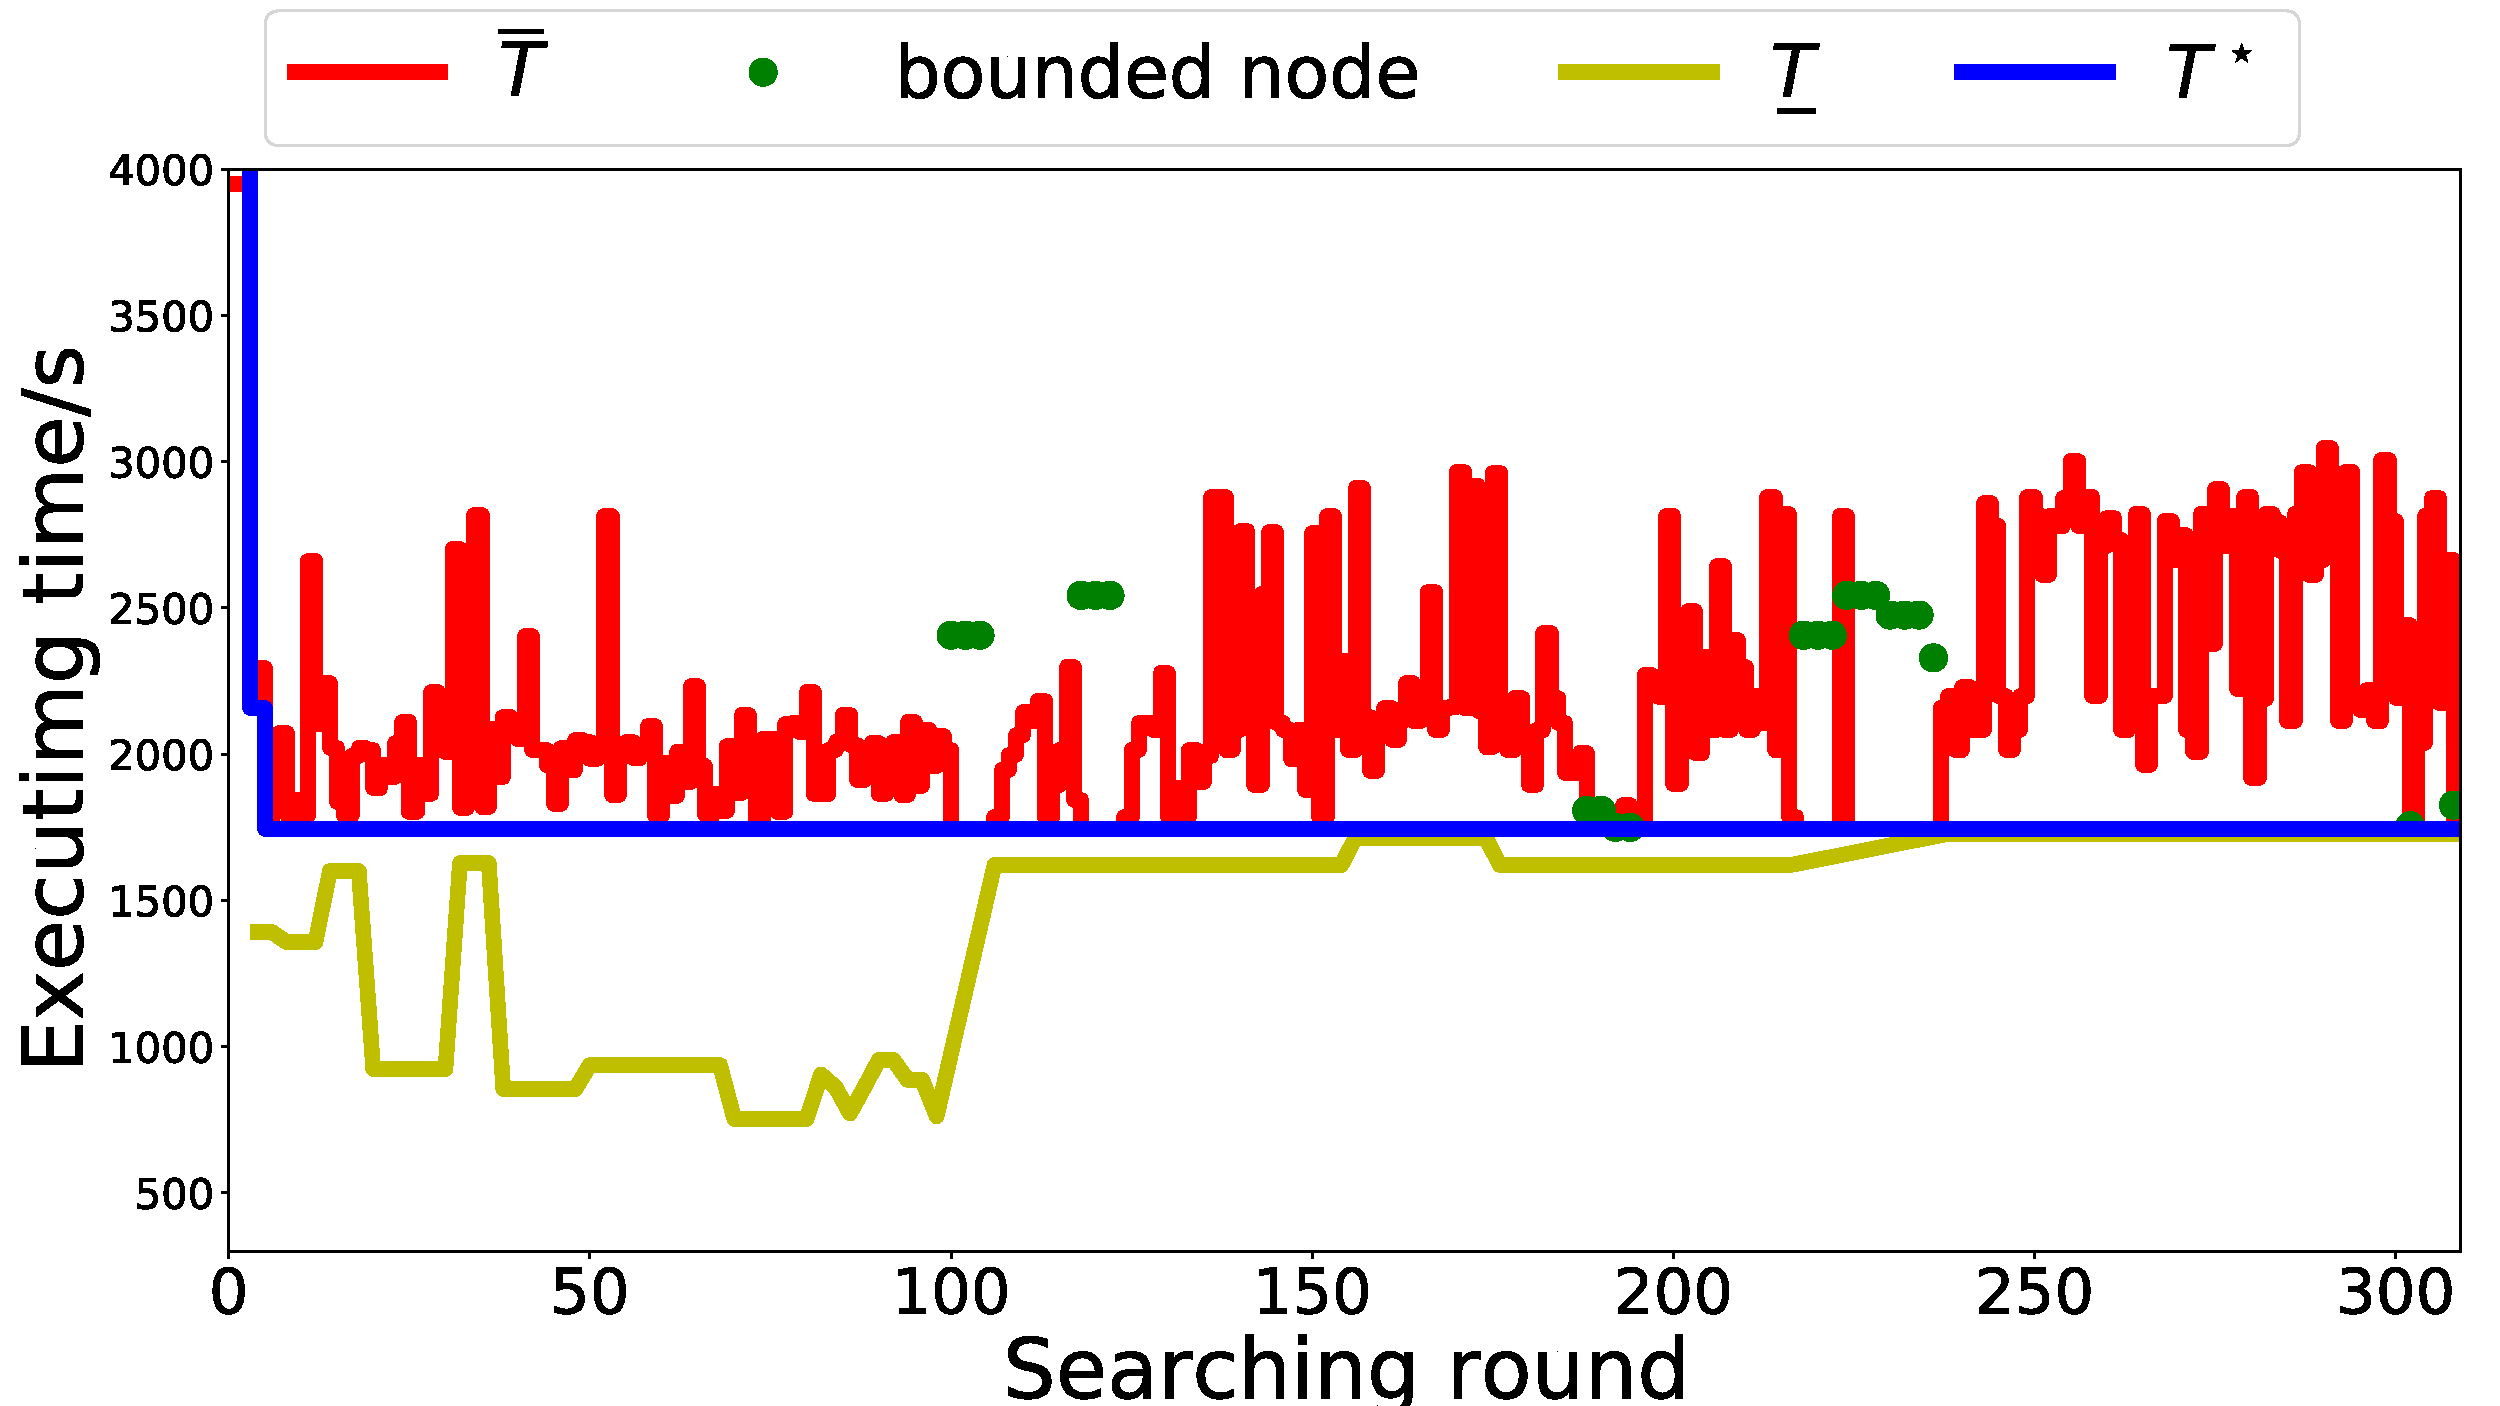
\includegraphics[width =0.5\textwidth]{figures/simulation/task2/bnb_search3.pdf}
\caption{ BnB search process of $\varphi_2$.}
\label{fig:hesse_task2}
\end{figure}

\begin{figure}[htbp]
		\centering
\includegraphics[width =0.45\textwidth]{figures/simulation/task2/gantt_graph.pdf}
\caption{Gantt graph of optimal task assignment in $\varphi_2$.}
\label{fig:gantt_task2}
\end{figure}

%==============================

%%========================================

%%========================================

%=========================================
\bibliographystyle{IEEEtran}
%=========================================
%%==============================
%==============================

\section{MILP Formulation}
Give a poset $P=(\Omega,\preceq_{\varphi},\neq_{\varphi})$, where $\Omega$ is a sequence of
subtasks, and~$\preceq_{\varphi}$, $\neq_{\varphi}$ are the partial relations
to describe the relative ordering between the subtasks.
Furthermore, $\omega_1\preceq_{\varphi}\omega_2$ means subtask $\omega_2$ should be
started after $\omega_1$ is started,
and $\omega_1\neq_{\varphi}\omega_2$ means that the execution of $\omega_1,\omega_2$ should not have intersection.
A team of agents is deployed to execute these subtasks under the constraints of
$\preceq_{\varphi},\neq_{\varphi}$ in the given workspace, e.g., as shown in Fig.~\ref{fig:workspace}.
Additionally, the agents are heterogeneous with three different types~$V_f,V_l,V_s$,
e.g., different velocities and functionalities.
For any subtask~$\omega_j\in\Omega$, it needs a particular combination of
different collaborators as specified in Table~\ref{fig:symbols}.
The objective function is to minimize the maximum execution time of
all subtasks in~$\Omega$, i.e., the makespan of the complete plan.
In particular, given the definition of variables in Table~\ref{tab:variables},
the Mixed Integer Linear Program (MILP) for solving this problem is formulated as follows.
Similar formulation can be found in~\cite{luo2021temporal, jones2019scratchs},
but with different objective function and different way of modeling the relative constraints.
The objective function is given by:
\begin{table}[t]
	\centering
	\caption{Description of related regions and agent actions.}
	\label{fig:symbols}
	\begin{tabular}{|c|m{0.5\columnwidth}|c|}\hline
		\textbf{Proposition} & \textbf{Description}\centering & \textbf{Duration} [s]\\ \hline
		$\texttt{p}_1,\cdots,\texttt{p}_{34}$ & $34$ PV panels. & $\backslash$ \\ \hline
		$\texttt{b}$ & Base stations for all agents to park and charge. & $\backslash$ \\ \hline
		$\texttt{t}_1,\cdots,\texttt{t}_7$ & $7$ transformers. & $\backslash$ \\ \hline
		$\texttt{temp}_{\texttt{p}_i,\texttt{t}_i}$ &
		Measure temperature of panel~$\texttt{p}_i$ and transformer $\texttt{t}_i$.
		Requires one~$V_f$. & 10 \\ \hline
		$\texttt{sweep}_{\texttt{p}_i}$& Sweep debris around any panel~$\texttt{p}_i$.
		Requires one $V_s$. & 190\\ \hline
		$\texttt{mow}_{\texttt{p}_i,\texttt{t}_i}$ &
		Mow the grass under panel~$\texttt{p}_i$ or transformer~$\texttt{t}_i$.
		Requires one $V_s$. & 190\\ \hline
		$\texttt{fix}_{\texttt{t}_i}$ &
		Fix malfunctional transformer~$\texttt{t}_i$.
		Requires one $V_l$ and one $V_s$ & 72\\ \hline
		$\texttt{repair}_{\texttt{p}_i}$ &
		Repair broken panel~$\texttt{p}_i$.
		Requires one $V_s$ to repair and two $V_f$ to guide. & 576\\ \hline
		$\texttt{wash}_{\texttt{p}_i}$ &
		Wash the dirt off panel~$\texttt{p}_i$.
		Requires one $V_l$ to wash and one $V_f$ to monitor the progress. & 565\\ \hline
		$\texttt{scan}_{\texttt{p}_i,\texttt{t}_i}$ &
		Build 3D models of panel~$\texttt{p}_i$ or transformer~$\texttt{t}_i$
		for inspection. Requires three $V_f$. & 95\\ \hline
	\end{tabular}
\end{table}
\begin{figure}
	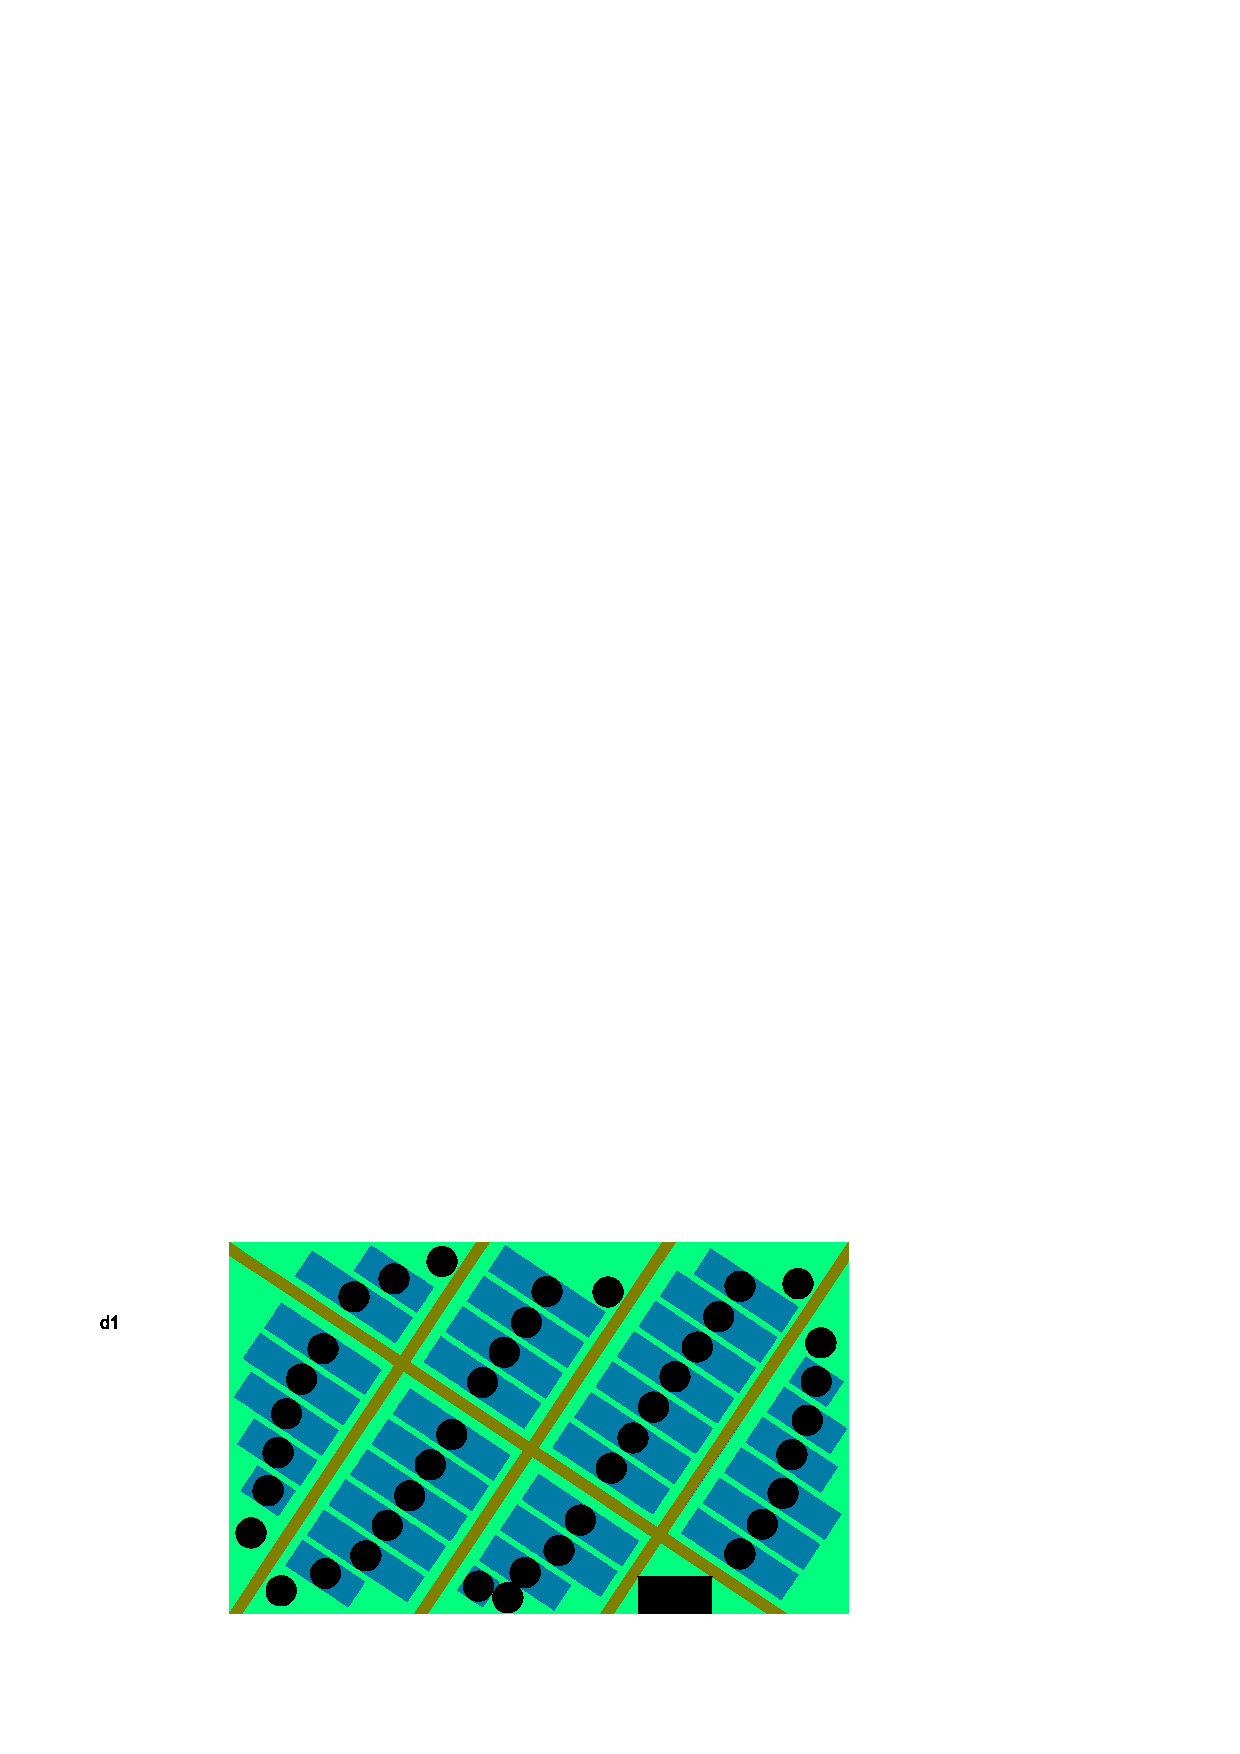
\includegraphics[width=0.36\textheight]{figures/background.pdf}
	\caption{The workspace layout of the simulated PV farm.}
	\label{fig:workspace}
\end{figure}

\begin{table}[t]
	\begin{tabular}{|l|p{0.5\columnwidth}|p{0.2\columnwidth}|}\hline
		Variable &\multicolumn{2}{c|}{ Variable definition }\\\hline
		Name & definition & range \\
		$P$ & partial order set& \\
		$m$  & number of agents & $\mathcal{N}$\\
		$n$ & number of tasks & $\mathcal{N}$ \\
		$i$ & agent $i$ & $i\leq n$\\
		$j$ & task $j$ & $j\leq m$	\\
		$k$ & order of tasks & $j\leq m$\\
		$o$ & number of serves type agent can provide & $ \mathcal{N}$\\
		$l$ & order of tasks & $j\leq o$\\
		$r$ & the ID of tasks set in $\neq$ & $\mathcal{N}$\\
		$\Omega$ & set of subtasks &\\
		$S^r$& a set of tasks belong to $\neq$ &\\
		$q^r_{j_1,j_2}$ &task $j_1$ execute in front of $j_2$ or not& $\{0,1\}$\\
		$T_b$ & a pretty large number as time budget & $T_b>0$ \\
		$r_{i,j,k,l}$ & agent $i$ execute task $j$ providing serve $l$ in the order $k$ & $\{0,1\}$\\
		$t_j$ & begin time of task $j$ & $t_j>0$ \\
		$p_j$ & continue time of task $j$ & $p_j >0$\\
		$a_{j,l}$ & number of servey $l$ task $j$ needed. & $\mathcal{N}$\\
		$b_{i,l}$ & type of servey $l$ that agent $i$ can provide & $\{0,1\}$ \\
		$v_i$ & velocity of agent $i$ &   $v_i>0$\\
		$dis_{j_1,j_2}$ & distance from task $j_1$ to task $j_2$ &  $dis_{j_1,j_2}>0$\\
		$dis_{i,j}$ & distance from initial $i$ to task $j$ & $dis_{i,j}>0$\\\hline
	\end{tabular}
	\centering
	\caption{Definition of variables used in the MILP.}
	\label{tab:variables}
\end{table}
\begin{equation}
\min_{r_{i,j,k,l}, t_j,q_{j_1,j_2}}  \max(t_j+p_j),
\label{0}
\end{equation}
is the objective function.
The following constraints should be satisfied.
Firstly, the $\preceq_{\varphi}$ constraints are enforced by
\begin{equation}
t_{j_1}+p_{j_1}\leq t_{j_2}, \quad  \forall (j_1,j_2)\in \preceq_{\varphi};
\label{1}
\end{equation}
the $\neq_{\varphi}$ constraints are enforced by:
\todoliu{update}
\begin{equation}
 t_{j_1}+p_{j_1}-q^l_{j_1,j_2}T_b\leq t_{j_2}, \forall S^l=\{j_1,j_2,\cdots,j_n\}\subseteq \neq_{\varphi}
 \label{1.5}
\end{equation}

\begin{equation}
\sum_{j_1,j_2\in S^l}q_{j_1,j_2} \leq |S^l|(|S^l|-1)-1, \forall S^l=\{j_1,j_2,\cdots,j_n\}\subseteq \neq_{\varphi}
\label{1.8}
\end{equation}

Furthermore, the required subtasks for each task~$j$ should be satisfied:
\begin{equation}
\sum_{i=1}^{m}\sum_{k=1}^{n}r_{i,j,k,l}b_{i,l}= a_{j,l},   \quad \forall j,l;
\label{2}
\end{equation}
Each agent can only provide the subtasks within its capability:
\begin{equation}
r_{i,j,k,l}\leq b_{i,l},   \quad \forall i,j,k,l;
\label{3}
\end{equation}
Each agent can execute one task no more than once:
\begin{equation}
\sum_{k=1}^{n}\sum_{l=1}^{o}r_{i,j,k,l} \leq 1,\quad   \forall i,j;
\label{4}
\end{equation}
Each agent at any time can execute no more than one task:
\begin{equation}
\sum_{j=1}^{m}\sum_{l=1}^{o}r_{i,j,k,l} \leq 1,\quad    \forall i,k;
\label{5}
\end{equation}
Each agent can execute $k+1$-th task only after it has executed $k$-th task:
\begin{equation}
  \sum_{j=1}^{m}\sum_{l=1}^{o}r_{i,j,k,l} - \sum_{j=1}^{m}\sum_{l=1}^{o}r_{i,j,k+1,l}
  \leq  0,    \quad\forall i,k<m-1;
\label{6}
\end{equation}
Each agent should obey its motion and action model:
\begin{equation}
\begin{aligned}
&t_{i_2}-t_{i_1} -M\sum_{l=1}^o r_{i,j_1,k,l}-M\sum_{l=1}^o r_{i,j_2,k+1,l}  \geq\\
& dis_{j_1,j_2}/v+p_{i_1}-2M, \quad   \forall i,j;
\end{aligned}
\label{7}
\end{equation}
\begin{equation}
t_{i} -M\sum_{l=1}^o r_{i,j,1,l} \geq dis_{i,j}/v-M, \quad  \forall i,j;
\label{8}
\end{equation}
With these constraints mentioned, the associated MILP is completed.
Unfortunately, the required number of bool variables
is $MN^2$, the complexity of solving the underlying MILP
is exploding as~$M$ and $N$ increase.



\section{Alternative Lower Bound}
\label{lower bound method}
In this section,
another method to compute the lower bound is proposed here,
which is more complex than the one proposed in the article.
But it can provide more accurate estimate of the lower bound,
particularly, it performs better when the number of agents and subtasks are small.
Instead of the original conditions in~\eqref{0}~\eqref{8},
a more relaxed version is used here.
More specifically, the distance cost is replaced by the time bound~$t_{low}$
as the minimum time for any agent to reach any goal region.
The lower bound consists of two parts:
the first part is to calculate the exact finishing time of all currently assigned tasks;
the second part is to estimate the makespan based on the current boundary condition.
In particular,
the set of used variables is summarized in Table~\ref{tab:variables2}.
Furthermore, the objective function is given by:
$$ \min_{t_{j_a}} \quad \max(t_{j_a}+p_{j_a}),$$
and the partial ordering constraints are given by:
\begin{equation}
t_{j_{a1}} + p_{j_{a1}}< t_{j_{a2}},   \quad \forall j_{a1}, j_{a2} \in P , j_{a1} \in N_a, j_{a2} \in N_a;
\label{9}
\end{equation}
when task $j$ is the first task of agent $i$, the motion constraint is given by:
\begin{equation}
dis_{i,j_a}/v_i+ p_{j_a}< t_{j_a};
\label{10}
\end{equation}
when task $j_{a2}$ is the subsequent task after task $t_{a1}$ of agent $i$,
the motion constraint is given by:
\begin{equation}
dis_{j_{a1},j_{a2}}/v_i+ p_{j_{a1}}+t_{j_{a1}}- t_{j_{a2}}<0;
\label{11}
\end{equation}
then $t_{i0}$ can be computed as the time each agent finishes
executing all assigned tasks
and starts to execute the remaining unassigned tasks.
$t_{j_a}$ is the time when the execution of task~$j_a$ is finished by agent~$i$.
Denote by~$T_i$ the set of tasks assigned to agent $i$, which yields the
computation of~$t_{i0}$ as follows:
\begin{equation}
t_{i0} = \max{\{t_{j_a}\}},    \quad {j_a}\in T_i;
\label{12}
\end{equation}

\begin{table}[t]
	\begin{tabular}{|l|p{0.5\columnwidth}|p{0.2\columnwidth}|}\hline
		Name & Variable definition & range \\\hline
		$P$ & partial order set& \\
		$M$  & number of agents & $\mathcal{N}$\\
		$\mathcal{M}$  & agent set & \\
		$N_a$ & set of assigned tasks &  \\
		$N_u$ & set of unassigned tasks &  \\
		$T_i$ & assigned tasks for agent $i$ &  \\
		$n_u$ & number of unassigned tasks & $\mathcal{N}$ \\
		$t_{j_a}$ & finished time of assigned tasks & $t_{j_a}>0$\\
		$\Omega$ & anchor function &\\
		$r_{i,j}$ & agent $i$ execute task $j$ & $\{0,1\}$\\
		$t_{i0}$ & begin time of agent $i$ & $t_i>0$ \\
		$t_i$ & end time of agent $i$ & $t_i>0$ \\
		$p_j$ & continue time of task $j$ & $p_j >0$\\
		$p'_j$ & estimate continue time of task $j$ & $p_j >0$\\
		$a_{j}$ & number agent task $j$ needed. & $\mathcal{N}$\\
		$v_i$ & velocity of agent $i$ &   $v_i>0$\\
		$dis_{j_1,j_2}$ & distance from task $j_1$ to task $j_2$ &  $dis_{j_1,j_2}>0$\\
		$dis_{i,j}$ & distance from initial $i$ to task $j$ & $dis_{i,j}>0$\\\hline
	\end{tabular}
	\centering
	\caption{variable definition}
	\label{tab:variables2}
\end{table}
For the remaining tasks, the final lower bound is modified by replacing the
task executing time~$p_j$ with the minimum possible motion cost~$p'_j$:
\begin{equation}
  p'_j = \min{\{\frac{dis_{i,j}}{v_i}, \frac{dis_{j_1,j_2}}{\max_i\, {v_i}}\}}+p_j,
  \quad \forall j\in N_u, \forall i \in \mathcal{M};
\label{13}
\end{equation}
Thus, the objective function and constrains are reformulated as follows:
\begin{equation}
\min_{r_{i,j},t_i} \;\max\, \{t_i\}
\label{14}
\end{equation}
the number of collaborators for each subtask is enforced by:
\begin{equation}
\sum_{i=1}^{m}r_{i,j} = a_{j},\quad  \forall j \in N_u;
\label{15}
\end{equation}
the relaxed constraint on motion and task executing time is given by:
\begin{equation}
\sum_{j=1}^{n}r_{i,j}p'_j +t_i > t_{i0}, \quad \forall i \in \mathcal{M},
\label{16}
\end{equation}
and $r_{i,j}$ is a boolean variable which is $1$ if task $j$ is assigned to agent $i$,
$0$ otherwise:
\begin{equation}
r_{i,j} \in\{0,1\}.
\label{17}
\end{equation}
The complexity of the first part is $O(N_a)$, while the complexity of
the second part is $O(N_u\cdot M)$.
Compared with~\eqref{0}, the ordering relations among subtasks are ignored
thus the poset constraint is neglected. In addition,
for each subtask, the constraints in \eqref{2}-\eqref{4} are removed
and only the constraint in~\eqref{15} is kept.
Also, a collaborative task is not required to be executed by the collaborators
at same time, thus the actual completion time is smaller.

\todoliu{
More specifically, let the current node be~$\nu$,
the set of unfinished subtasks is given by~$\Omega^-_\nu$ in~\eqref{eq:node-tasks}.
The first lower bound~$\underline{T}_{\nu,1}$ on the makespan
to accomplish~$\Omega^-_\nu$ is computed via analyzing the poset
graph~$\mathcal{G}_{P_\varphi}=(\Omega,\, E,\, R)$ in~\eqref{def:poset-graph}.
In particularly, consider the directed
graph~$\mathcal{G}'_{P_\varphi}=(\Omega'_\nu,\, E\cap R )$,
where~$\Omega'_\nu$ is the set of nodes associated with the unfinished subtasks,
and the set of edges contains the edge $(\omega',\,\omega)$ that belongs to
both~$\preceq_{\varphi}$ and~$\neq_{\varphi}$.
Then, starting from the set of root nodes that does not have parent nodes,
a BFS procedure is used to traverse all nodes in the graph~$\mathcal{G}'_{P_\varphi}$.
Denote by~$\Gamma^-_{\nu}=\{\tau_{\omega_f,\omega_g}\}$ the set of paths
from any root node~$\omega_f$ to any other node~$\omega_g$ in the graph.
Then, the first lower bound~$\underline{T}_{\nu,1}$ on the makespan is given by
\begin{equation}\label{eq:lower-bound-1}
\underline{T}_{\nu,1} (\nu,\,P_{\varphi})=\textbf{max}_{\tau\in \Gamma^-_\nu} \, \{T_{\tau}\},
\end{equation}
where~$T_{\tau}$ is the accumulated duration
of path~$\tau=\omega_0\omega_1\cdots \omega_P$, i.e., $T_\tau=\sum_{p=1}^PT_{\omega_p}$.
In other words, the lower bound~$\underline{T}_{\nu,1}$ assumes that
there are as many agents as needed for the sub-tasks, while the partial ordering
constraints for the subtasks are ensured.
Secondly, another lower-bound~$\underline{T}_{\nu,2}$ is estimated by
ignoring the partial ordering constraints:
\begin{equation}\label{eq:lower-bound-2}
\underline{T}_{\nu,2} (\nu,\,P_{\varphi})=\frac{\sum_{\omega\in \Omega^-_{\nu}}
	T_{\omega} N_{\omega}}{N},
\end{equation}
where~$T_{\omega}$ and~$N_{\omega}$ are the duration and number of agents required
for subtask~$\omega\in \Omega^-_\nu$ as defined in~\eqref{eq:node-makespan}.


Consequently, the lower bound on the makespan of all solutions rooted from~$\nu$
is given as the minimum of these two lower bounds above:
\begin{equation}\label{eq:lower-bound}
\underline{T}_\nu = \texttt{lower\_bound}(\nu,\,P_{\varphi})
= \min\,\{\underline{T}_{\nu,1},\, \underline{T}_{\nu,2}\},
\end{equation}
which can be computed efficiently.
It is worth noting that the task assignments associated with~$\underline{T}_\nu$
above is infeasible as it either violates the partial ordering constraints or
the current agent capacities.

}


\section{Details for Numerical Simulation}
\subsection{Planner and Controller}
Each agent is governed by a two-level path planner:
the high-level planner relies on the $A^\star$ method to find the
discrete sequence of waypoints from any initial position to the goal position;
the low-level planner is a simple P-controller with~$RVO$ for collision avoidance.
The agent synthesizes the discrete path first with high level planner,
then uses the lower-level planner to navigate the robot between waypoints.
The transition function between the regions is different among the agents, e.g.,
the UAV can move freely without considering any obstacles,
while the UGVs are restricted from the areas around the PV panels and off-road obstacles.
The collision avoidance mechanism via~$RVO$ is only activated
when the distance between any two agents is smaller than a threshold.

There are three types of agents: $V_f$, $V_s$, $V_l$:
$V_f$ is a quadrotor with model Crazyflie $2.0$,
which has a onboard navigation controller.
All UAVs have the same height and can only move in the $x,y$ plane;
$V_s, V_f$ are both four-wheel-driven car with  MecanNum wheels, with
a simple onboard navigation controller for rotation and translation.


\subsection{Additional Figures}
This section contains the figures illustrating the simulation results
in Section VIII-A,
of the original article, which were omitted for lack of space.

Fig.~\ref{fig:poset_graph1}-\ref{fig:gantt_task1} are the poset graph, the BnB search process,
and the final execution plan for task~$\varphi_1$;
while Fig.~\ref{fig:poset_graph2}-\ref{fig:gantt_task2} are for task~$\varphi_2$.
\begin{figure}[htbp]
		\centering%
		\includegraphics[width =0.18 \textwidth]{figures/simulation/task1/ipe_poset_graph.pdf}
		\caption{Poset graph of task $\varphi_1$. }
                \label{fig:poset_graph1}
\end{figure}

\begin{figure}[htbp]
	\centering
	\includegraphics[width =0.45\textwidth]{figures/simulation/task1/bnb_search1.pdf}
	\caption{ BnB search process of $\varphi_1$.}
        \label{fig:hesse_task1}
\end{figure}

\begin{figure}[htbp]
		\centering
\includegraphics[width =0.43\textwidth]{figures/simulation/task1/gantt_graph.pdf}
\caption{Gantt graph of optimal task assignment in $\varphi_1$.}
\label{fig:gantt_task1}
\end{figure}

%===========================

\begin{figure}[htbp]
		\centering%
\includegraphics[width =0.3\textwidth]{figures/simulation/task2/ipe_poset_graph.pdf}
\caption{Poset graph of task $\varphi_2$.}
\label{fig:poset_graph2}
\end{figure}

\begin{figure}[htbp]
		\centering
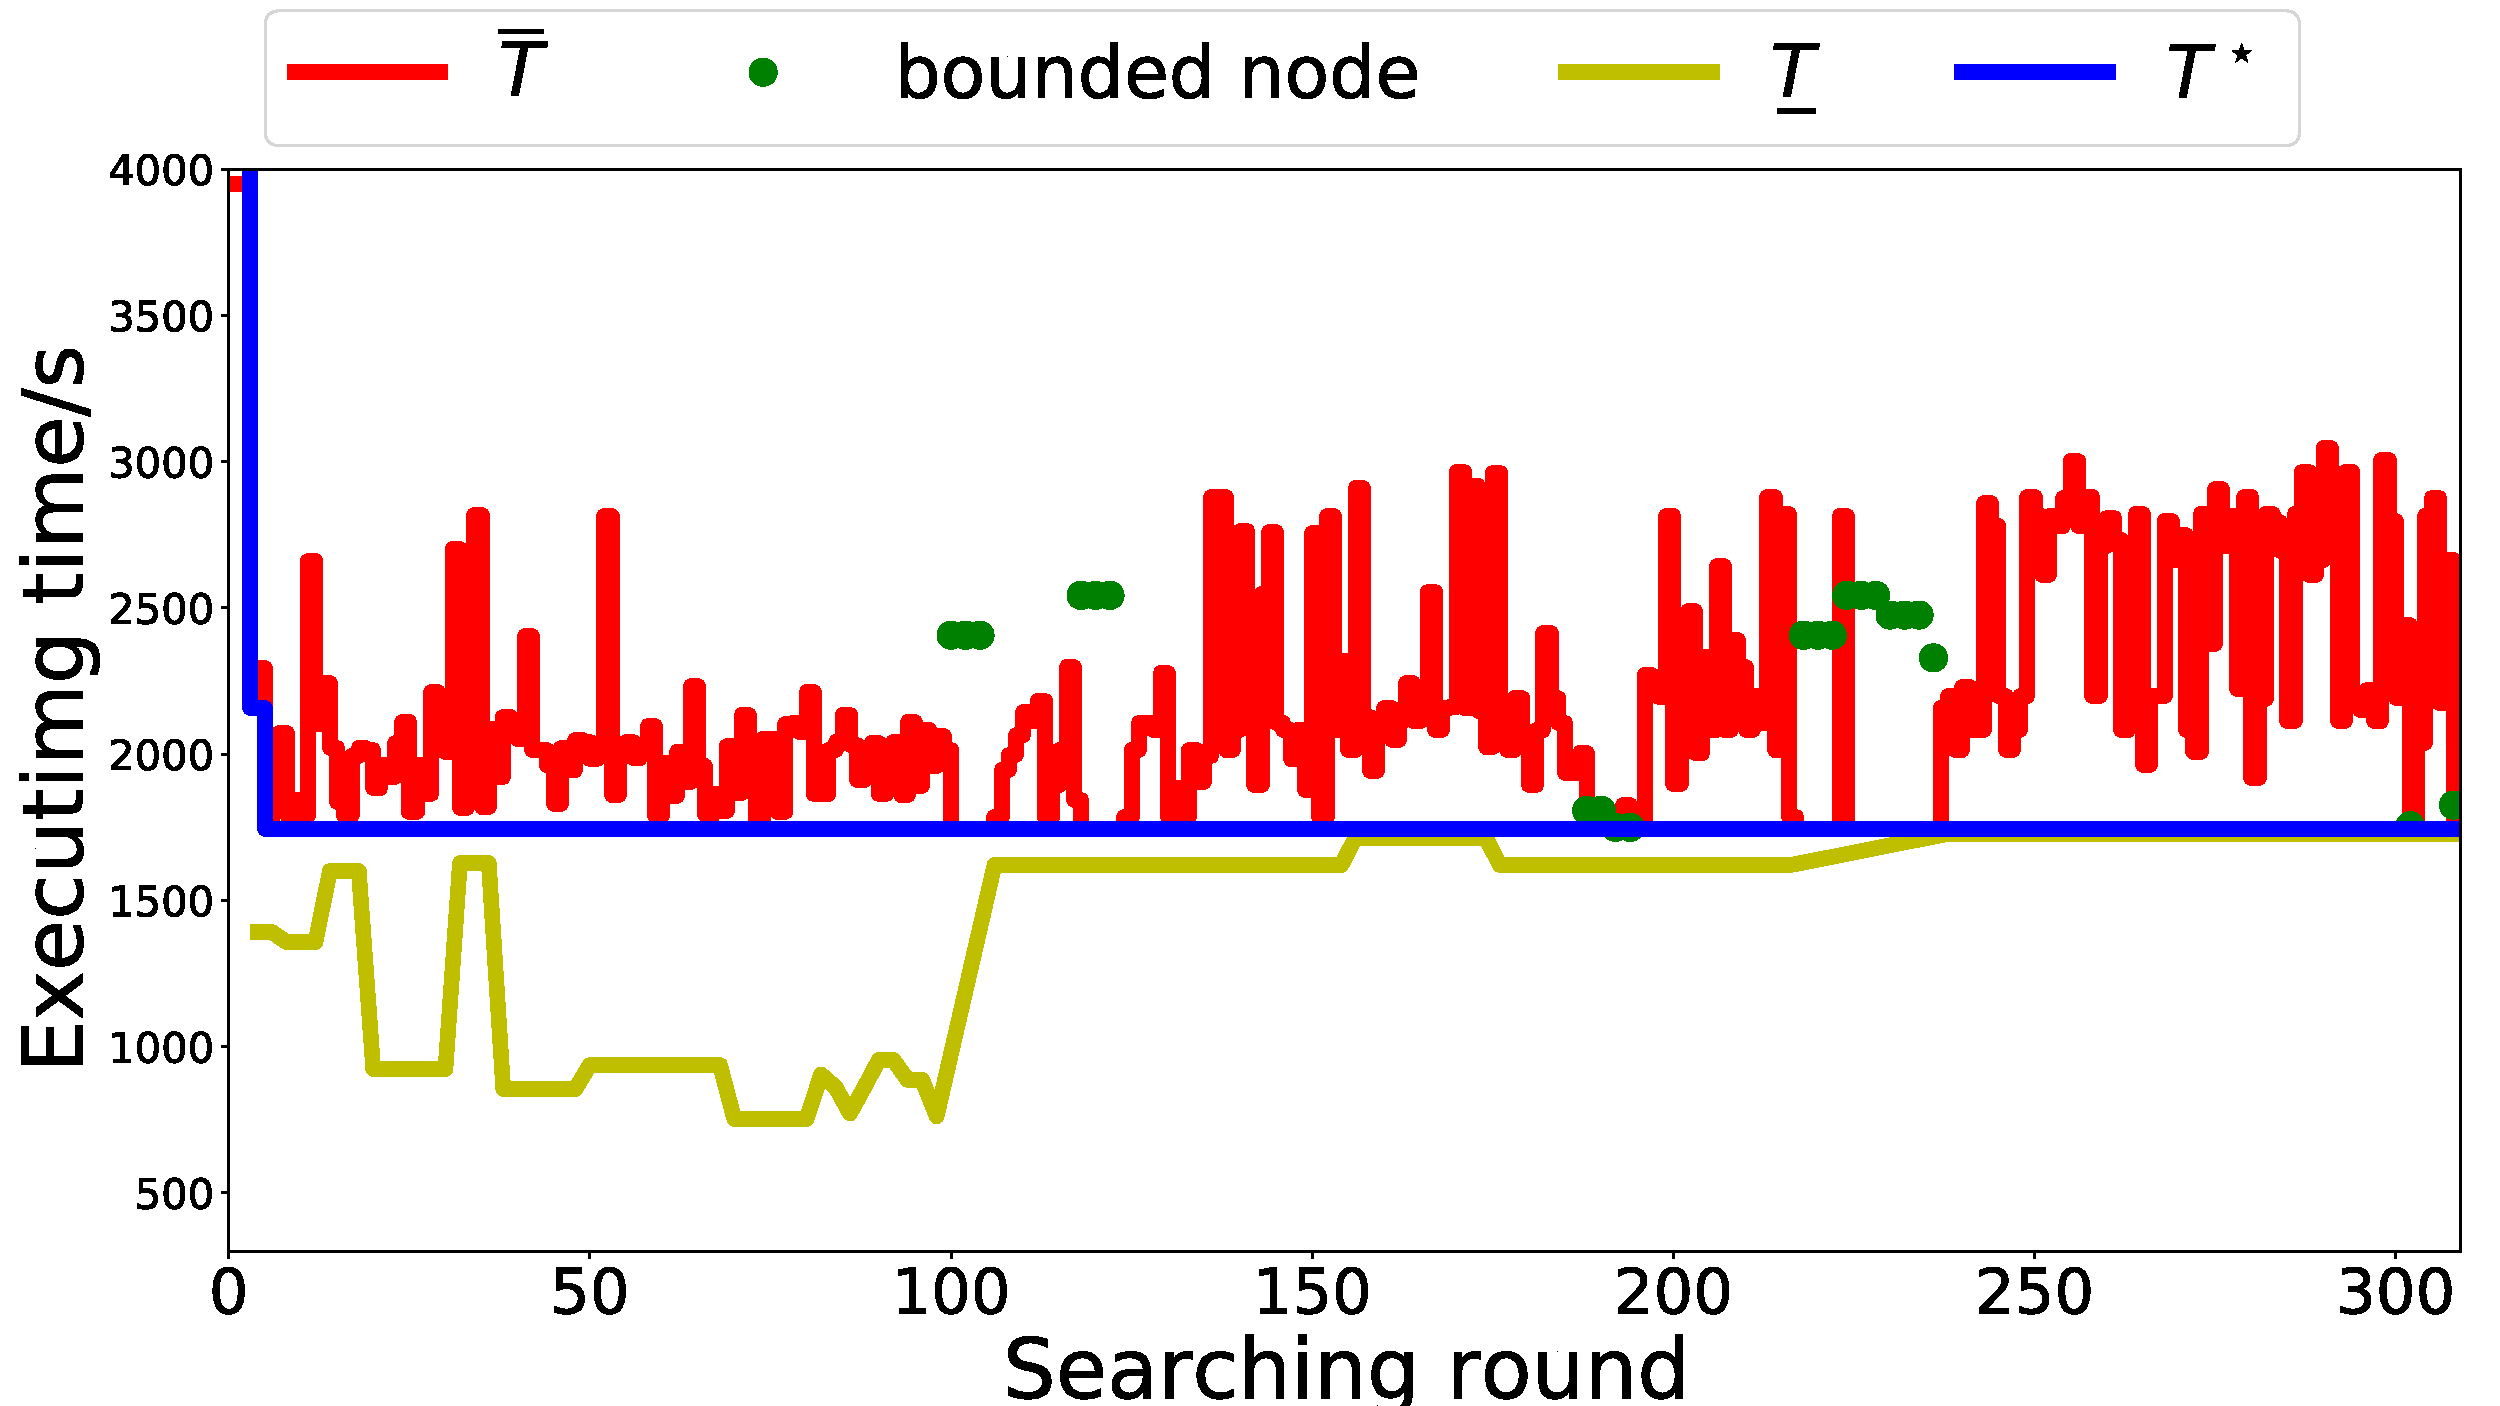
\includegraphics[width =0.5\textwidth]{figures/simulation/task2/bnb_search3.pdf}
\caption{ BnB search process of $\varphi_2$.}
\label{fig:hesse_task2}
\end{figure}

\begin{figure}[htbp]
		\centering
\includegraphics[width =0.45\textwidth]{figures/simulation/task2/gantt_graph.pdf}
\caption{Gantt graph of optimal task assignment in $\varphi_2$.}
\label{fig:gantt_task2}
\end{figure}

%==============================

\end{document}
